\chapter{Einleitung}
\section{NP-Vollst�ndigkeit}
Eine Sprache B ist \textbf{NP-Vollst\"andig} wenn gilt:
\begin{enumerate}
	\item $B \in NP$
	\item $\forall A \in NP: A \prec_p B$
\end{enumerate}

Notiz:\\
$A \prec_p B$ : $A$ ist polynomialzeitreduzierbar auf $B$

\section{Polynomialzeitreduktion}
Eine Sprache $A$ ist polynomialzeitreduzierbar auf Sprache $B$, $A \prec_p B$, wenn eine in polynomialer Zeit berechenbare Funktion $f:\Sigma^* \to \Sigma^*$ existiert, f�r die gilt:\\
$\forall w:$
	$w \in A \iff f(w) \in B$

Die Funktion $f$ hei�t dann Polynomialzeitreduktion von $A$ nach $B$.

\section{Definition 3SAT}
Spezialform des Erf\"ullbarkeitsproblems
\begin{itemize}
	\item Literal:\\
	$x_i$ oder $\overline{x_i}$
	\item Variable:\\
	$x_i$ (l: Anzahl der Variablen)
	\item Klausel:\\
	$(x_1 \lor \overline{x_2} \lor \overline{x_3} \lor x_4)$ (k: Anzahl der Klauseln)
	\item CNF-Formel(cnf-formula - conjunctive normal form):\\
	$(x_1 \lor \overline{x_2} \lor \overline{x_3} \lor x_4) \land (x_3 \lor \overline{x_5} \lor x_6) \land (x_3 \lor \overline{x_6})$
	\item $\phi$: $(x_1 \lor \overline{x_2} \lor \overline{x_3}) \land (\overline{x_2} \lor x_4 \lor ...) \land ... \land (\overline{x_3} \lor ... \lor ...)$
\end{itemize}

$3SAT = \left\{ \right. \langle \phi \rangle | \phi$ ist eine erf�llbare 3CNF-Formel$\left. \right\}$

$\phi = 1 \iff \forall c_j$: mindestens ein Literal ist $true$ 

\chapter{Hamilton-Pfad-Problem}
\section{Definition}
\begin{itemize}
	\item Geht durch jeden Knoten genau einmal
	\item Startet in s
	\item Endet in t
\end{itemize}

Notiz: Gesucht: Pfad von $s$ nach $t$, der durch jeden knoten genau einmal geht.

\section{Beweis Gerichtet}
\subsection{Konstruktion von G}
$\phi \to G$

\subsubsection{Darstellung Variable $x_i$}
\begin{center}
	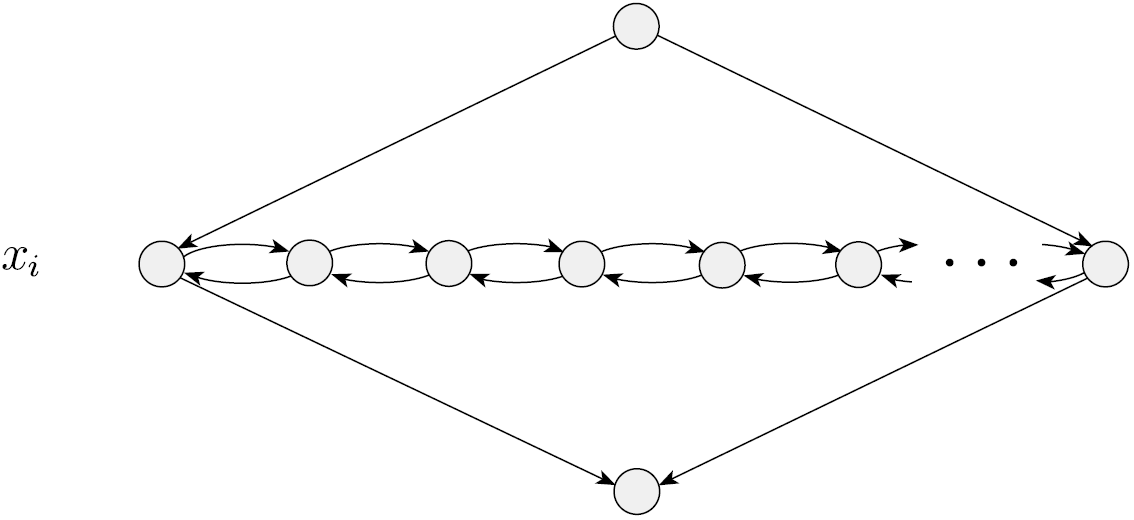
\includegraphics[width=14cm]{images/hampath/1}
\end{center}

\subsubsection{Darstellung Klausel $c_j$}
\begin{center}
	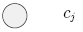
\includegraphics{images/hampath/2}
\end{center}

\subsubsection{High-level structure of G}
\begin{center}
	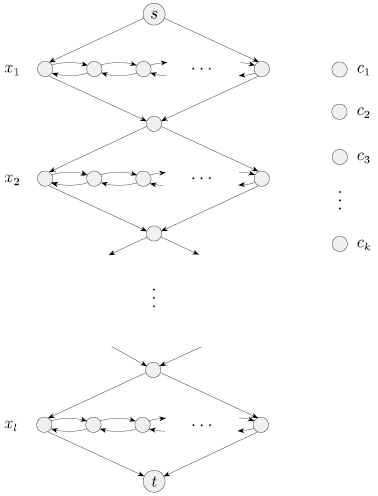
\includegraphics[width=14cm]{images/hampath/3}
\end{center}

\subsubsection{Horizontale Struktur im Diamant}
\begin{center}
	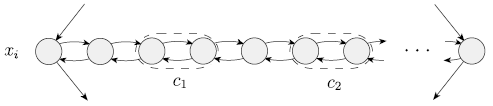
\includegraphics[width=14cm]{images/hampath/4}
\end{center}
$\left<3k+1\right>$ Knoten

\subsubsection{Zus\"atzliche Kanten wenn $x_i$ in $c_j$ ist}
\begin{center}
	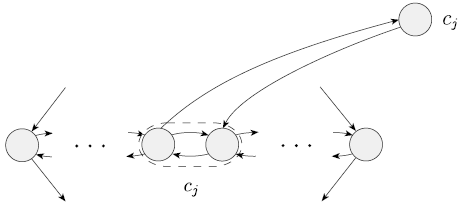
\includegraphics[width=14cm]{images/hampath/5}
\end{center}

Notiz: Am Beispiel von $\phi$ zeigen!

\subsubsection{Zus\"atzliche Kanten wenn $\overline{x_i}$ in $c_j$ ist}
\begin{center}
	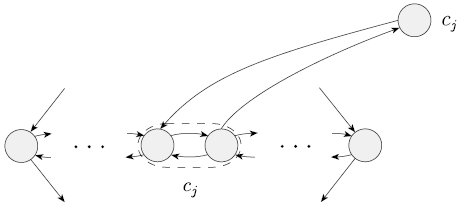
\includegraphics[width=14cm]{images/hampath/6}
\end{center}

\subsection{$\phi$ ist erf\"ullbar}

Notiz: Zun\"achst werden die Knoten $c_j$ ignoriert.

Notiz: Der Pfad geht von $s$ nach $t$ durch jeden Diamanten nach einander.

Notiz: Um alle Knoten zu treffen muss der Pfad entweder zig-zaggen oder zag-ziggen.

\subsubsection{Zig-zagging and Zag-zigging}
\begin{center}
	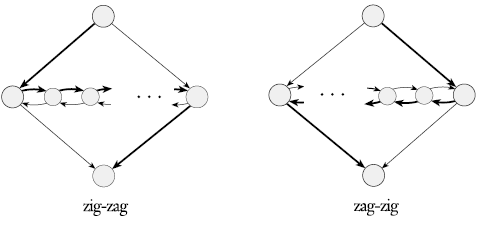
\includegraphics[width=14cm]{images/hampath/7}
\end{center}

Notiz: Zig-zagging wenn Variable $x_i=true$, Zag-zigging wenn Variable $x_i=false$

Notiz: Jetzt fehlen nurnoch die Knoten $c_j$.

Notiz: In jeder Klausel $c_j$ w\"ahlen wir einen Literal aus, dem wir $true$ zuweisen.

Notiz: Jeder wahre Literal in einer Klausel ist nur eine Option f�r einen Umweg \"uber einen Klauselnoten. $\to$ Es wird immer nur ein Umweg zu jedem Klauselknoten genommen. $\to$ Knostruktion von $G$ ist beendet.

\subsubsection{This situation cannot occur}
\begin{center}
	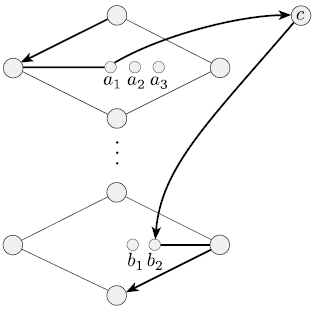
\includegraphics[width=14cm]{images/hampath/8}
\end{center}

\subsubsection{Laufzeit}
Notiz: Offentsichlich nicht polynomial

\subsection{Ungerichtet}
\TODO{muss der auch rein?}

\chapter{SUBSET-SUM-Problem}
\section{Definition}
\begin{itemize}
	\item Integer-Arithmetik
	\item Menge von Nummern: $x_1,...,x_k$
	\item Ziel $t$
	\item Kann $t$ durch eine Teilmenge erreicht werden?
\end{itemize}

\section{Beweis}
3SAT $\prec_p$ SUBSET-SUM

$\phi:$ Boolesche Formel\\
$x_1, x_2,...,x_l$
$c_1, c_2,...,c_k$ Teilausdr\"ucke

\subsection{Gesucht}
$\prec_p: \phi \mapsto \left<S,t\right>$

$\phi: (x_1 \lor \overline{x_2} \lor x_3) \land (x_2 \lor x_3 \lor ...) \land ... \land (\overline{x_3} \lor ... \lor ...)$

Notiz: $c_1, c_2, c_k$ dran schreiben

\subsection{Annahme}
Es existiert eine Konfiguration f�r die $\phi$ erf\"ullt ist.

$\Rightarrow$ Subset bauen\\
	$y_i$ iff $x_i=true$ else $z_i$
	
$\Rightarrow$ $t=11...1133...33$\\
Notiz: l mal $1$ und k mal $3$

$\Rightarrow$ F\"uge solange $g_i$ unf $h_i$ hinzu bis das Target t erreicht ist.

\begin{tabular}{c | c c c c c c | c c c c}
 & 1 & 2 & 3 & 4 & ... & l & $c_1$ & $c_2$ & ... & $c_k$ \\
\hline
$y_1$ & 1 & 0 & 0 & 0 & ... & 0 & 1 & 0 & ... & 0 \\ 
$z_1$ & 1 & 0 & 0 & 0 & ... & 0 & 0 & 0 & ... & 0 \\
$y_2$ &   & 1 & 0 & 0 & ... & 0 & 0 & 1 & ... & 0 \\
$z_2$ &   & 1 & 0 & 0 & ... & 0 & 1 & 0 & ... & 0 \\
$y_3$ &   &   & 1 & 0 & ... & 0 & 1 & 1 & ... & 0 \\
$z_3$ &   &   & 1 & 0 & ... & 0 & 0 & 0 & ... & 1 \\
... &   &   &   &   & ... &   &   &   & ... &   \\
$y_l$ &   &   &   &   &  & 1 & 0 & 0 & ... & 0 \\
$z_l$ &   &   &   &   &  & 1 & 0 & 0 & ... & 0 \\
\hline
$g_1$ &   &   &   &   &  & 1 & 0 & 0 & ... & 0 \\
$h_1$ &   &   &   &   &  & 1 & 0 & 0 & ... & 0 \\
$g_2$ &   &   &   &   &  &   & 1 & 0 & ... & 0 \\
$h_2$ &   &   &   &   &  &   & 1 & 0 & ... & 0 \\
... &   &   &   &   & ... &   &   &   & ... &   \\
$g_k$ &   &   &   &   &  &   &   &   &  & 1 \\
$h_k$ &   &   &   &   &  &   &   &   &  & 1 \\
\hline
\hline
t & 1 & 1 & 1 & 1 &... & 1 & 3 & 3 & ... & 3\\
\end{tabular}

Notiz: Zeigen, dass $\phi$ erf\"ullbar ist mit einem subset von S dass sich auf t summiert.

Notiz: $\forall c_j:$ Mindestens eine Variable von $c_j$ muss $1$ sein, da maximal $2$ von $g_j$ und $h_j$ kommen k\"onnen.

Notiz: $\phi=true$ iff $\forall c_j: c_j=true$ 
$\Rightarrow$ reduzierbar

\subsection{Laufzeit}
Tabelle hat etwa eine Gr\"o�e von $(l + k)^2$\\
Jeder Eintrag ist leicht zu berechnen $\Rightarrow O(n^2)$